\documentclass[12pt]{scrartcl}
\usepackage[spanish]{babel}
\usepackage{graphicx} % Required for inserting images
\usepackage{amsmath}
\usepackage{float}



\title{Plantilla \LaTeX}
\author{Laura del Mar Jerez}
\date{\today}



%_____________________________________
\begin{document}
\maketitle
\tableofcontents
\newpage


\begin{abstract}
    Aqui hay que poner un resumen de qué va el documento \ldots
\end{abstract}

\section{Introduction}
\subsection{Texto}
\label{sec:intro}In March 2006, Congress raised that ceiling and additional \$0.79 trillion to \$8.97 trillion, which is approximately 68\% of GDP. As of October 4, 2008, the ``Emergency Economic Stabilization Act of 2008" raised the current debt ceiling to \$11.3 trillion.

\begin{itemize} %no numerada
    \item No numerada
\end{itemize}

\begin{enumerate} %numerada
    \item esta si
    \item aqui hago referencia a la seccion \ref{sec:intro} jejejej
\end{enumerate}

\subsection{Fórmulas}

a = b + c

$ \mu = b_2 + c^{2+3} $

$\Omega=\sum_{k=1}^{n}\omega_k$

\subsubsection*{Formula cuadrática}
 Aqui tenemos la fórmula cuadrática
\begin{equation}
\label{eq:Cuadratica}
   x = \frac{-b \pm \sqrt{b^2 -4ac}}{2a} 
\end{equation}



\subsection{Ecuaciones}
aqui referencio a la cuadratica \eqref{eq:Cuadratica}
\begin{equation}
    x = \frac{-b \pm \sqrt{b^2 -4ac}}{2a}
\end{equation}


\begin{equation*}
    x = \frac{-b \pm \sqrt{b^2 -4ac}}
    {2a}
\end{equation*}

\begin{align*} %entorno aling // salto de linea y & separa la columna despus del signo =
(x+1)^3 & = (x+1)(x+1)(x+1)\\
&= (x+1)(x^2 + 2x + 1)\\
&= x^3 + 3x^2 + 3x +1
\end{align*}

\subsection*{Texto y ecuaciones} 
Sea $X_1, X_2, \ldots, X_n$ una sucesión de variables aleatorias independientes e idénticamente distribuidas con $E[X_i] = \mu $ y $Var[X_j] = \sigma^2 < \infty $, y sea 

\begin{equation}
    S_n = \frac{1}{n}\sum^n_iX_i
\end{equation}

su media. Entonces, cuando $n$ tiende a infinito, las valiables aleatorias $\sqrt{n}(S_n - \mu)$ convergen a una distribución normal $N(0,\sigma^2).$

\section{Formulas}
\begin{figure}[H]  % [H] indica que se debe colocar aquí la imagen
    \centering
    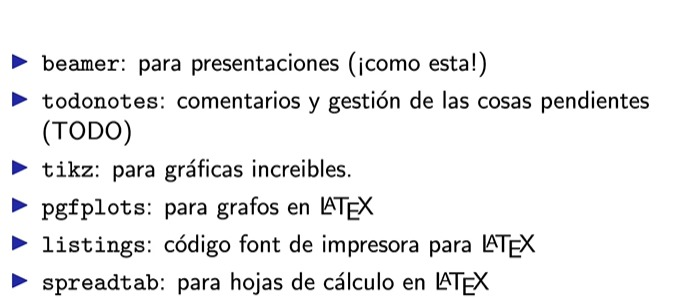
\includegraphics[width=0.5\linewidth]{Curso/metodos.jpg}
    \caption{Caption}
    \label{fig:enter-label}
\end{figure}



\end{document}
